\chapter{Theory}
\label{2-teorie}

\section{Web Processing Services}

The Web Processing Service (WPS) is an Open Geospatial
Consortium (OGC) standard that provides rules for publishing and
executing processes on the web. „The standard also defines how a
client can request the execution of a process, and how the output from
the process is handled. It defines an interface that facilitates the
publishing of geospatial processes and clients’ discovery of and
binding to those processes. The data required by the WPS can be
delivered across a network or they can be available at the server.“
\cite{wpsstandard}

%% ML: tady michate hrusky a jabka (HTTP je protokol, XML je jazyk),
%% ale nechme to prozatim tak jak to je
%% ML: Jedna zkratka je vysvetlena, druha ne
%% JP: Zkratky upraveny

\zk{WPS} uses \zk{HTTP} (Hypertext Transfer Protocol) and \zk{XML} (eXtensible Markup Language) for describing
processes and data transfer. The first version 0.4.0 was released in
2005. Despite a new version 2.0.0 having been released in 2015,
version 1.0.0 remains most widely used.

A process is essentially a function p that returns an output Y for
each input X:\\ \centerline{p: X $\rightarrow$ Y}

In case of \zk{WPS}, a process is a geospatial operation, calculation or a
model of any complexity. It may require one or more input arguments
and always yields one or more outputs. If there are no input
arguments, the process is either generating constant or random
values. While \zk{WPS} was designed for geospatial data, it is not
restricted to them.

\begin{figure}[H] \centering
  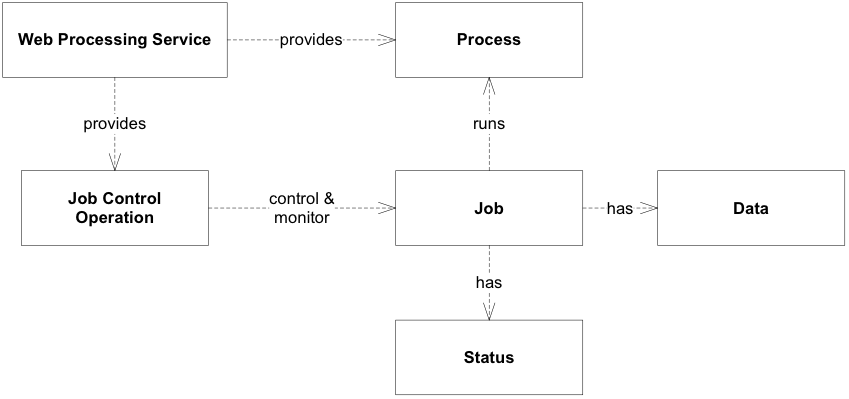
\includegraphics[width=400pt]{./pictures/wps_conceptual_model.png}
  %% ML: zdroj je standard? Potom uvedte cely nazev standardu? Zkratka nestaci
  %% JP: opraveno, zdroj je dokumentace OGC
      \caption[WPS conceptual model]{WPS conceptual model (source: \href{http://docs.opengeospatial.org/is/14-065/14-065.html\#10}{Open Geospatial Consortium})}
      \label{fig:WPS}
  \end{figure}

There are two basic capabilities of a \zk{WPS} server. It provides the
process and retrieves the process description and it controls and
monitors processing jobs. Job is an instance of a process – it is an
object created for a particular process execution. Job control is the
ability to execute, dismiss or delete a job.

\subsection{Process execution}


There are two ways in which a process can be executed. If the
complexity of the process is lower, the connection is stable and the
completion time is relatively short (for instance, the Apache2 server
uses 60 seconds as a default value for ConnectionTimeout \cite{apache})
the execution is run synchronously. After the execute request is sent
by the client, the \zk{WPS} server starts executing the process while the
client remains connected to the server for the entire time of the
execution. Only when the process has finished and the output has been
delivered, the connection terminates.

The asynchronous execution, on the other hand, better suits for
complex processes that are expected to take longer time to
finish. When the client requests process excecution, the server
responds with a status information message that confirms the request
has been accepted and the process will be run. The message also
includes a unique processing job identifier. Then, the connection is
interrupted. At this time, the client can send a GetStatus request
with the job identifier to get information on how the process has
progressed. Once the process has finished, the client can access the
output data using a GetResult request with the job identifier. The
asynchronous execution can be also useful in case of unstable
connection that prevents synchronous execution to successfully run.

\subsection{Available operations}

\textbf{GetCapabilities.} A mandatory operation for any \zk{OGC} Web
service. \cite{getcap} For \zk{WPS}, it is one of the three basic operations that are
available for any process. There are no input parameters required. Once
the request is sent, the server returns a document that includes
information about the service provider, a list of operations available
for a \zk{WPS} server and a list of all the processes offered by the
service.

\noindent \textbf{DescribeProcess.} Another basic operation. The only
required input is the name (or a list of names) of the process to be
described. \cite{despro} If the process offers description in multiple languages, a
language parameter can be added to the request. It returns a document
with characteristics of the process and a description of input
parameters. It also describes the output format of the process.

\noindent \textbf{Execute.} The key operation for any \zk{OGC} \zk{WPS}
service. It allows processes that are implemented by a server to be
run. \cite{execute} It requires input parameter values as specified by the
service. These can be either values (numerical or other) that are
included directly in the request or references to other recources that
are accessible as local files or through the web. Analogically,
outputs of the execute operation can be included in the \zk{XML}
response document or stored locally or on the web. In case of asynchronous
operation, the response contains a unique JobID that the client uses
to enquire about the process status and results.

\noindent \textbf{GetStatus.} An operation only used for asynchronous
processes. After the Execute request has been accepted, the client can
use this operation to query status information of the processing job,
using a JobID returned by the Execute response. \cite{getstat} This operation is only
available in version 2.0.0.

\noindent \textbf{GetResult.} The final operation used for
asynchronous processes that is to be used after the GetStatus
operation reports the process has finished. The input parameter is the
unique JobID. \cite{getres} Then, GetResult fetches the results of the process as
described in the Execute section. This operation is only available in
version 2.0.0.

\noindent \textbf{Dismiss.} Allows the client to let the server know
the result of the process is no longer wanted. In such case, all the
resources corresponding to the JobID sent in the Dismiss request may
be deleted. \cite{dismiss} If the process is still running, it may be cancelled. This
operation is only available in version 2.0.0.

\subsection{OGC\ WPS Implementations}

%% ML: itemize -> subsection
%% JP: upraveno
\subsubsection{PyWPS}
\begin{figure}[H] \centering
      
\includegraphics[width=200pt]{./pictures/pywps.png}
      \caption[PyWPS logo]{PyWPS (source:
\href{http://pywps.org/images/pywps.png}{PyWPS})}
      \label{fig:PyWPS}
  \end{figure}

PyWPS is a server side implementation of the OGC Web Processing
Service (\zk{OGC} \zk{WPS}) standards 1.0.0. It is written in the Python
programming language, it runs on Python 2.7, 3.3 or higher and it is
tested and developed on Linux. \cite{pywpsinfo} It uses a ConfigParser format for
configuration files.\cite{pywpsconf} It supports a variety of geospatial software and
tools such as GRASS \zk{GIS}, R Project or the \zk{GDAL} library. Synchronous
and asynchronuous invocations are supported. As for request encoding,
two options are available - key-value pairs (using HTTP-GET) or \zk{XML}
payload (using HTTP-POST). Every process that is to be deployed on the
server is defined as a class and has several mandatory parameters. The
key parameter called "handler" gets invoked every time there is an
incoming request, it accepts the request and returns a response.

In 2016, it upgraded from PyWPS 3 to PyWPS 4. Some of the more
significant changes include every input being considered a list of
inputs and all inputs having file, data and stream attributes. \cite{pywps3to4} These
attributes allow better manipulation with data.
	
As PyWPS only supports version 1.0.0 of the OGC \zk{WPS} standards, it does
not support operations implemented in version 2.0.0. These operations
are GetStatus, GetResult and Dismiss. Support for version 2.0.0 is
currently being planned.\cite{pywps}
 

\subsubsection{ZOO-Project}
\begin{figure}[H] \centering
      
\includegraphics[width=200pt]{./pictures/zoo.png}
      \caption[ZOO-Project logo]{ZOO-Project (source: ZOO-Project)}
      \label{fig:ZOO-Project}
  \end{figure}

ZOO-project is an open source \zk{WPS} platform that consists of several
components. The core processing engine, ZOO-Kernel, is a \zk{WPS} server
written in C that implements \zk{WPS} standards 1.0.0 and 2.0.0.\cite{zoo}
A significant advantage over other \zk{WPS} implementations is that it is
written as a polyglot, i.e. in a valid form of multiple programming
languages, which performs the same operations independent of the
programming language used to compile or interpret it.\cite{polyglot}
It runs on Mac OS, Linux and Microsoft Windows operating systems. It
uses a ConfigParser styled configuration file.

ZOO-services offers a rich collection of ready-to-use services that
are built on open source libraries such as \zk{GDAL} or GRASS \zk{GIS}.

ZOO-API is a server-side library written in JavaScript for creation
and chaining services. These services can be written in one of five
programming languages that are supported. It also offers easy
conversion of vector formats.

ZOO-Client is a simple client-side JavaScript \zk{API} for interacting with
\zk{WPS} from web applications. It allows to build \zk{WPS} requests and send
them to a \zk{WPS} server. \cite{zooclient} It also provides functions to easily parse the
output \zk{XML} responses.


\subsubsection{52°North WPS}
\begin{figure}[H] \centering
      
\includegraphics[width=150pt]{./pictures/52n.png}
      \caption[52° North logo]{52 North (source: 52° North)}
      \label{fig:52 North}
  \end{figure}

52°North \zk{WPS} is a part of the 52°North open source software
initiative. Located in Germany, their aim is to foster innovation in
the field of geoinformatics through a collaborative process. As a part
of this inititiave, the 52°North \zk{WPS} is an implementation of the \zk{OGC}
\zk{WPS} standard (version 1.0.0). It is written in the Java programming
language. It can be run under Linux or Microsoft Windows operating
systems.

As for the \zk{WPS} invocation methods, it supports both synchronous and
asynchronous invocation, HTTP-GET and HTTP-POST. As for the WPS
datatypes, it supports GeoTIFF, Shapefile, \zk{KML}, \zk{WKT} and
others. \cite{north} Configuration is based on an \zk{XML} file.
  

\subsubsection{ESRI Web Processing}

\begin{figure}[H] \centering
      
\includegraphics[width=200pt]{./pictures/esri.png}
      \caption[ESRI logo]{ESRI (source: ESRI)}
      \label{fig:ESRI}
  \end{figure}

ESRI is an international company oriented on desktop and mobile \zk{GIS}
software, geodatabases and web \zk{GIS}. Founded in 1969, it is the leading
company in the global \zk{GIS} market. It offers a variety of \zk{GIS} products,
including ArcGIS for Desktop, ArcGIS Online or ArcGIS for Mobile.

It allows services created within the ArcGIS software to be published
and shared online on another ESRI's platform, ArcGIS Server. \cite{esripublish} On ArcGIS
Server, these services can be stored and accessed by other users. They
can be also implemented alongside with maps, which can also be created
in other ArcGIS software and then published online, into online web
applications. Users can also take advantage of the Web App Builder
feature and of many templates that simplify creating applications.

By default, ESRI software does not follow \zk{WPS} standards. However, when
publishing a geoprocessing service in ArcGIS Desktop, there is a
possibility to enable the \zk{WPS} capability. Then, the service published
is compliant with the \zk{OGC} \zk{WPS} 1.0.0 specifications.\cite{arcgiswps}

\section{Spatial Databases}

Spatial database (or a geodatabase) is a database optimized for
storing and querying data related to objects in geometric space, such
as points, lines or polygons. They require additional functionality
for processing spatial data effectivelly. Usually, special data types
such as geometry or feature are added along standard data types. In
addition to typical SQL queries such as SELECT statements, spatial
databases can perform a wide variety of spatial operations. These
spatial operations include (but are not restricted to) computing line
length, polygon area, distance between geometries, etc.

The International Organization for Standardization (\zk{ISO}) and \zk{OGC} specify a
Simple Features standard that is divided into two parts. The first one
defines a general model for two-dimensional geometries. \cite{sfa} It also deals
with spatial reference systems. The second part defines an
implementation using SQL. This second part is implemented to varying
extent in most of spatial databases and extensions. \cite{sfa}

Here I list the best known and most widely used spatial database
systems, however, there are many more. In fact, most of the major
database systems support spatial data, including Microsoft \zk{SQL} Server
or MySQL (and its community developed branch MariaDB). Also, there is
a number of database systems especially designed and developed as
spatial databases (e.g. SpatialDB, SpaceBase, MapD).

\subsection{PostGIS} \label{postgis}
\begin{figure}[H] \centering
      
\includegraphics[width=190pt]{./pictures/postgis.png}
      \caption[PostGIS logo]{PostGIS (source: PostGIS)}
      \label{fig:PostGIS}
  \end{figure}
  
PostGIS is an open-source spatial database extension for
PostgreSQL. \cite{pstgis} PostgreSQL is a widely-used object-relational database
management system. PostGIS adds support for geographic objects
according to the \zk{OGC} Simple Features for \zk{SQL} specification.

PostgreSQL and PostGIS use the client/server architecture. \cite{postgre} When a
client makes a request (typically an \zk{SQL} statement), there is a server
that accepts and evaluates it. The server itself is then responsible
for updating (or, generally, changing in any way) the database
file. Two of the most significant advantages of PostgreSQL over other
\zk{DBMS}s are its high standard compliance and extensibility. It allows
"stored procedures" to be created and saved to simplify complex
operations that are frequently repeated.

In a study that compared PostGIS with Oracle Spatial, PostGIS was
found to perform faster when accessing and querying
data. \cite{postgis}

	
\subsection{Oracle Spatial and Graph}

\begin{figure}[H] \centering
      
\includegraphics[width=200pt]{./pictures/oracle.png}
      \caption[Oracle logo]{Oracle (source: Oracle)}
      \label{fig:Oracle}
  \end{figure}
  
  
The Oracle Spatial and Graph is an extension of the Oracle Database
that allows managing geographic data in a native type within an Oracle
database. It is also a client-server service \cite{oraclearch} but, unlike PostGIS, it
is proprietary. Spatial features extend Oracle Locator, a standard
feature of the Oracle Database distribution. Oracle Locator provides
basic functions and services in Oracle Spatial but it lacks more
advanced functions. Oracle Spatial and Graph supports large-scale
geographic information systems, provides spatial web services and
generally is designed for complex spatial data management and
analysis.

\subsection{SpatiaLite}

\begin{figure}[H] \centering
      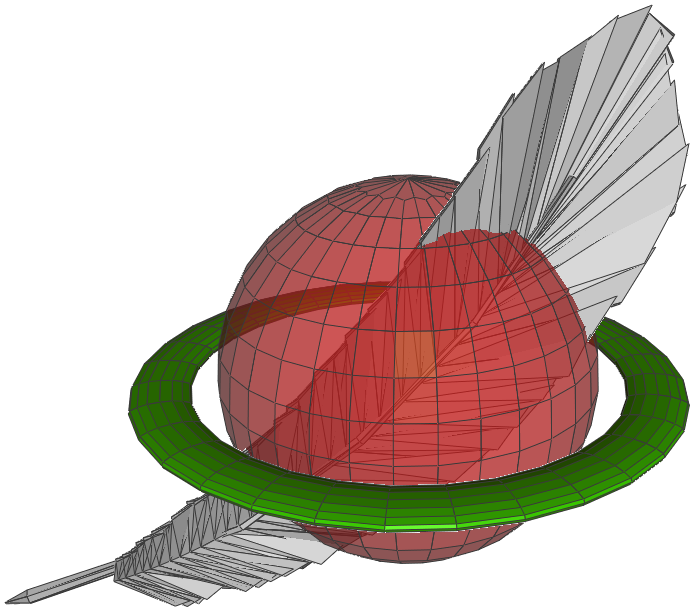
\includegraphics[width=150pt]{./pictures/spatialite.png}
      \caption[SpatialLite logo]{SpatialLite (source: SpatialLite)}
      \label{fig:SpatialLite}
  \end{figure}
  
SpatiaLite is a lightweight library that extends the SQLite database
management system so it provides support for spatial data. Unlike
Oracle and PostgreSQL, SQLite is designed as a single file-based database. \cite{sqlitefile} It
means that, unlike server-based databases, by using SQL expressions a
user updates the file directly. Therefore, a file-based database must
be stored in the local file system. As a consequence, SQLite is very
fast and efficient for standard operations but is not optimized for
multi-user applications or for large-scale operations. SQLite (and
SpatiaLite) is open-source. \cite{sqliteopen}

\subsection{ArcSDE \& Geodatabase (ESRI)}

\begin{figure}[H] \centering
      
\includegraphics[width=170pt]{./pictures/arcsde.png}
      \caption[ArcSDE logo]{ArcSDE (source: ArcSDE)}
      \label{fig:ArcSDE}
  \end{figure}
	
ESRI is a supplier of a wide range of \zk{GIS} software, including web \zk{GIS}
services, desktop and mobile applications and geodatabase management
systems. Data used, produced or derived from ESRI software is stored
in geodatabases, that are defined by ESRI as "a collection of
geographic datasets of various types held in a common file system
folder, a Microsoft Access database, or a multiuser relational
DBMS."\cite{esridef} As the definition suggests, ESRI distinguishes
between three conceptually different types of geodatabases, depending
on the scale of the data, requirements of the client, operating system
and other factors.

In its simplest form, an ESRI geodatabase can be a collection of GIS
data stored as files in a folder within the standard file system. This
is called file geodatabase and is intended for single users and small
workgroups. Personal geodatabase is another type of geodatabase, also
designed to be used by individuals or small workgroups. It uses
Microsoft Access database management system and therefore is only
available on Microsoft Windows operating system.

The final and most complex type of geodatabase is the enterprise
geodatabase. Unlike the previous two, it is designed to be used by
multiple users simultaneously and for large datasets. It works with
various \zk{DBMS}s storage models using ArcSDE.

ArcSDE is a proprietary technology for managing and accessing spatial
data that supports multiple \zk{DBMS}s: IBM DB2, IBM Informix, Microsoft \zk{SQL}
Server, Oracle, and PostgreSQL.\cite{arcsdedoc} It also supports the
corresponding standards. ArcSDE is built with the client/server
architecture. A client first sends a request to the server. Then, the
server receives the request, generates results, and delivers them to
the client.

\begin{figure}[H] \centering
      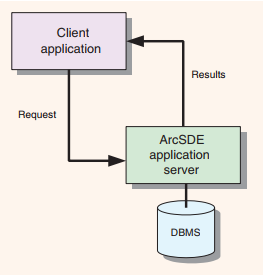
\includegraphics[width=200pt]{./pictures/arcsdeobr.png}
      \caption[ArcSDE logic]{ArcSDE logic(source: ArcSDE)}
      \label{fig:ArcSDE logic}
  \end{figure}

The client doesn't need any knowledge of particulars of any of the
\textbf{DBMS}s. Another significant advantage is that ArcSDE allows datasets to
be available to multiple users for viewing, querying or editing at the
same time.\cite{esritypes}

\section{Background research}


PyWPS is only one of the many implementations of the \zk{WPS} standard,
each of them approaching the problem of storing output data
differently. From those listed above, the ZOO-project provides the
"ZOO-kernel optional database support" \cite{zoodb} that is most
similar to what the author of this thesis is aiming to create. There
is an optional section in the configuration file that allows to
configure the connection. The section has six elements (dbname, port,
user, host, type and schema) that are used to generate a connection
string that is passed to the GDAL library that connects to the
database.\cite{zoodbsec}

When using ArcGIS Server (ESRI software for executing processes on a
server), ArcSDE handles storing data in a database. For more
information about the ArcSDE technology, refer to the section 2.2.4 -
ArcSDE \& Geodatabase (ESRI).

As for the 52°North Web Processing Service, it, by default, stores output data as
web accessible resources and provides the consumer with an
URL. Depending on the type of the output data, it may be stored
directly as \zk{WMS}, \zk{WFS} or \zk{WCS} layers. \cite{north} 

As an alternative, it is also possible to store the data within a PostgreSQL database. \cite{52north} It is, however, primarily used to save requests and responses, e.g. to help debugging the service. While storing output data in the database is technically possible, too, no spatial database is implemented at the moment.\footnote{Information obtained from personal email correspondence with Benjamin Proß, the contact person for 52°North WPS}